%\documentclass[twoside,openright,a4paper,11pt]{book}
%
%
\usepackage[utf8]{inputenc}
\usepackage[francais]{babel}
\usepackage[T1]{fontenc}

\addto\captionsfrench{\def\tablename{\textsc{Tableau}}}% pour avoir TABLEAU et pas TABLE dans les légendes des tableaux

%%%%%%% MISE EN PAGES %%%%%%
\usepackage{geometry}
\geometry{outer=2cm,inner=3cm,top=3cm}

\setcounter{tocdepth}{3}     % Dans la table des matieres
\setcounter{secnumdepth}{3}  % Avec un numero.
\usepackage{setspace}

\usepackage{fancyhdr}	% marge en haut et en bas
\pagestyle{fancy}

\fancyhead{}	% vide l'entête
\fancyfoot{} % vide le pied~de~page

\fancyhead[RO]{\leftmark}
\fancyhead[LE]{\rightmark}
\fancyfoot[C]{\thepage}	% numéro de page en bas au centre

\renewcommand{\headrulewidth}{0.4pt} % épaisseur du trait en haut
\renewcommand{\footrulewidth}{0.4pt} % épaisseur du trait en bas

\fancypagestyle{mypagestyle}{%
    \fancyhead{}	
    \fancyfoot{} 
    \fancyfoot[C]{\thepage}
    \renewcommand{\headrulewidth}{0.4pt} 
	\renewcommand{\footrulewidth}{0.4pt} 
}

\fancypagestyle{couvertureAbstract}{%
    \fancyhead{}	
    \fancyfoot{} 
    \fancyfoot[C]{}
	\renewcommand{\headrulewidth}{0pt} 
	\renewcommand{\footrulewidth}{0pt} 
}
%
\usepackage{layout}
\usepackage{tocbibind} % include tableofcontent in itself

%%%%%% PAGE DE GARDE %%%%%%

\geometry{outer=2cm,inner=3cm,top=3cm}
\usepackage[scaled]{helvet} % font used on cover (Helvetica)
\usepackage{eso-pic} % to set background picture
\usepackage{multicol} % for back cover (abstracts)
\usepackage{graphicx} % to include logos
\usepackage{tikz} % to compose background picture

% Colors (extracted from SPI's template)
\definecolor{boxcolor1}{rgb}{0.91373,0.92941,0.87451}
\definecolor{boxcolor2}{rgb}{0.94902,0.93333,0.91373}
\definecolor{boxcolor3}{rgb}{0.76078,0.87843,0.17647}
\definecolor{headercolor}{rgb}{0.94118,0.30980,0.17255}
\definecolor{namecolor}{rgb}{1.0,0.4,0.0}
\definecolor{titlecolor}{rgb}{0.19216,0.51765,0.60784}
% Also used: gray, teal (predefined by xcolor package, usually loaded by document class)

% Cover environment, to keep changes local
\newenvironment{cover}{%
  \fontfamily{phv}\selectfont % Select Helvetica font
  \pagestyle{empty} % No page number
}{
  \addtocounter{page}{-1}
  \cleardoublepage
}

% Macro for background common to front and back
\newcommand{\tikzBG}{%
  \path (0,0) rectangle (1,1);
  %TODO: You should adjust the bottom height of the following rectangle to fit your abstract's length
  \path [fill=boxcolor1] (.0571,.11) rectangle (.481,.963); 
  \path [fill=boxcolor2] (.4333,.697) rectangle (.9048,.7475);
  \path [fill=boxcolor2] (.4333,.7811) rectangle (.9048,.8316);
  \path [fill=boxcolor2] (.4333,.8687) rectangle (.9048,.9192);
  \path [fill=boxcolor3] (.0571,.7879) rectangle (.5762,.8316);
  \node[inner sep=0pt] at (0.2285,0.8788) [above left] {%
    
\includegraphics[height=.0707\paperheight,keepaspectratio]{./figures/logo/logo_unb.png}};
  \node[inner sep=0pt] at (0.6667,0.8788) [above right] {%
    
\includegraphics[height=.0808\paperheight,keepaspectratio]{./figures/logo/logo_ecn_color.png}};
  \node at (.0571,.8316) [above right,color=headercolor] {%
    \fontsize{29}{35}\selectfont\bfseries Th\`ese de Doctorat};
}

% Macro for repeated information (to avoid insconsistency)
%TODO: fill in with no formatting but desired case
\newcommand{\firstName}{Jean-Rémy}
\newcommand{\surname}{Gloaguen}
\newcommand{\thesisTitle}{Estimation du niveau sonore de sources d'intérêts au sein de mixtures sonores urbaines : application au trafic routier}

%%%%%%% SYMBOLES %%%%%
\usepackage{tipa}	% pour avoir l'accent concave
\usepackage{lmodern}	% pour les guillemets
\usepackage{gensymb}	% pour les degrés
\usepackage{enumitem}	% pour changer le symbole de l'item (\begin{itemize}[label=$\bullet$])

%%%%%%% EQUATION %%%%%%
\usepackage{amssymb}
\usepackage{amsmath}
\usepackage{fancybox}
\usepackage{xfrac}	% fraction de type "1/4"
\usepackage{cases}	% système équation
\usepackage[overload]{empheq}
\usepackage{bm}		% pour mettre en gras .
\usepackage{units} 	% x/y barre latérale pour les fractions
%
%%%%%%% FIGURE %%%%%%
\usepackage{subfigure}	% utiliser subfigure
\usepackage{float}	% utiliser H dans les figures
%
%%%%%% TABLEAUX %%%%%%
\usepackage{array,multirow,makecell}
%\addto\captionsfrench{\def\tablename{\textsc{Tableau}}}% pour avoir TABLEAU et pas TABLE dans les légendes des tableaux
\usepackage{colortbl} % pour avoir des lignes colorées dans les tableau
%\usepackage{slashbox} % pour les \backslashbox
%\usepackage{subcaption}
\usepackage{hhline}	% pour les lignes horizontales 
\usepackage{tabularx} % permet itemize dans les cellules
\usepackage{booktabs}
\usepackage{longtable}	% pour les tableaux longs

\newcolumntype{L}[1]{>{\raggedright\let\newline\\\arraybackslash\hspace{0pt}}m{#1}}
\newcolumntype{C}[1]{>{\centering\let\newline\\\arraybackslash\hspace{0pt}}m{#1}}
\newcolumntype{R}[1]{>{\raggedleft\let\newline\\\arraybackslash\hspace{0pt}}m{#1}}

%%%%% ALGORITHME %%%%%
\usepackage{algorithm}
\usepackage{algorithmic}

%%%%% BIBLIO %%%%%
\usepackage[fixlanguage]{babelbib}
\selectbiblanguage{french}
\usepackage{breakcites}	% pour couper les références en bout de ligne

%%%%% APPENDICES %%%%%%%
\usepackage[toc,page]{appendix}

%%%%%%%%%%%%%%%%%%%%%
\usepackage{url}	% gérer les adresses www.
\linespread{1.2}	% interligne

\cleardoublepage
%
%\begin{document}

\chapter{Connaitre l'environnement sonore urbain : de la prédiction à la mesure}
\thispagestyle{empty}

\section{Pourquoi s'intéresser à l'environnement sonore urbain ?}

Au sein de l'Union Européenne, 70 $\%$ de la population, soit quasiment 340 millions d'habitants, vivent dans des zones urbaines \cite{europ-commission_data_2017}. 486 villes concentrent chacune plus de 100 000 habitants. En France, selon l'INSEE, c'est même plus de 84 $\%$ de la population qui vivent dans une zone urbaine, soit plus de 55 millions d'habitants. Cette concentration soulève de grandes questions autour de l'organisation de l'espace urbain afin d'offrir une qualité de vie acceptable aux citadins. En effet avec de telles densités (environ 3000 habitants/km$^2$ et jusqu'à plus de 21 000  habitants/km$^2$ pour la ville de Paris, la plus dense de l'UE) plusieurs formes de pollutions viennent dégrader l'environnement urbain. Des sources de désagrément perçues par le citadin, le bruit est le phénomène qui provoque le plus de gène après la pollution de l'air. Ce bruit est le fruit des activités humaines, provenant essentiellement du transport qu'il soit routier, ferroviaire ou aérien \cite{zannin_characterization_2013}.\\

Selon un rapport de l'Organisation Mondiale de la Santé \cite{who_burden_2017}, en Europe, près de 200 millions de personnes sont exposées quotidiennement à des niveaux sonores supérieurs à 55 dB(A), soit 40$\%$ de la population. Près de 20 $\%$ atteignent même plus de 65 dB(A) en journée et plus de 30 $\%$ sont touchés par un niveau sonore excédant 55 dB(A) la nuit. En France, selon un rapport de l'ADEME \cite{europeens2016analyse}, ce sont 52 millions de personnes qui se disent affectés par le bruit et principalement le bruit de trafic routier. Plus de 7 millions d'individus y sont alors exposés à des niveaux supérieur à 65 dB(A) au quotidien et à plus de 55 dB(A) la nuit.
Cette exposition quotidienne, à de tel niveaux, n'est pas dans conséquence pour l'Homme. L'impact sur l'organisme humain à l'exposition du bruit est observé et étudié depuis de nombreuses années \cite{ising1980health}. Parmi les effets possibles les plus courant sont des troubles du sommeil \cite{pirrera2010nocturnal}, de la vigilance et de la concentration, l'augmentation du stress, de la pression artérielle et du rythme cardiaque \cite{babisch2008road, babisch2005traffic}. En conséquence, selon le rapport de l'OMS, se sont près de 8 millions de personnes en Europe qui sont affectés par des troubles du sommeil mais aussi 900 000 touché par de l'hypertension. On estime aussi que 43 000 hospitalisations sont imputables au bruit dues à des pertes de vigilance et de concentration  et jusqu'à 10 000 cas de mort prématurés par an. Cet impact sur la santé n'est pas sans conséquence entraînant un coût financier pour la société : en France, ce coût est estimé à plus de 11,5 milliard d'euros par an dont une grande partie (89 $\%$) est imputable au bruit du trafic routier \cite{europeens2016analyse}. 

De plus, si le bruit en ville impact la vie des citadins, celui-ci se fait également ressentir auprès de la faune sauvage \cite{dutilleux_anthropogenic_2012, francis2009noise} en leur causant également du stress ou en compliquant la communication et la reproduction entre les individus. Les conséquences du bruit sur l'écosystème ne doivent donc pas être ignoré.\\

Le bruit et une trop grande exposition à celui-ci a donc un impact négatif sur les Hommes et sur leur environnement. C'est donc un enjeu de société dont les français ont conscience \cite{JNA2016etude}. 
Il est donc nécessaire et utilise de s'intéresser aux ESU afin de mieux connaitre la répartition du bruit et comment le citadin perçoit cet environnement.
La plupart des mesures prises se focalisent sur le bruit de trafic puisqu'il est la sources la plus gênante. 

De nombreux modèles numériques existent afin de pouvoir prédire les niveaux sonores émis par du trafic routier \cite{quartieri2009review}, ferroviaire \cite{van2000railway} et aérien \cite{zaporozhets1998aircraft}.
A partir de ces modèles, est instauré en 2002, dont le but est de mieux connaitre la répartition du bruit émanant de ces principales sources de bruit en ville ainsi que des Installations Classées pour la Protection de l'Environnement ICPE dans les agglomérations de plus de 100 000 habitants. Cette directive prévoit

\begin{itemize}
	\item d'évaluer l'exposition au bruit des populations basée sur des méthodes communes aux pays européens,
	\item d'informer les populations sur leur niveau sonore d'exposition et sur les effets du bruit sur la santé,
	\item de connaitre et de délimiter les zones bruyantes et les zones calmes.\\
\end{itemize}

Cette directive prévoit notamment la production de cartes de bruits stratégiques qui permettent alors de cibler les endroits où le niveau sonore est élevé pour ainsi réaliser des aménagements qui permettront de le réduire (construction d'un mur anti-bruit, réduction de la vitesse, mise en place d'un revêtement sol particulier).


\section{Réaliser des cartes du bruit en ville}
Mises à jours tout les 5 ans, les cartes de bruit résument, pour chaque source de bruit, les niveaux sonores globaux moyens pondérés $A$ sur 24h ($L_{DEN}$ pour \textit{Day-Evening-Night}) et durant la nuit ($L_N$) : 

\begin{equation}
L_{DEN} = 10\times\log \left(\frac{1}{24} \left(12\times10^{\frac{L_D}{10}}+4\times10^{\frac{L_E+5}{10}}+8\times10^{\frac{L_N+10}{10}} \right)\right)
\end{equation} 

avec $L_D$, $L_E$ et $L_N$, les niveaux sonores moyens à long terme pondéré A respectivement pour les périodes 6h-18h, 18h-22h, 22h-6h (ou bien 23h-7h suivant le rythme de vie du pays), 

\begin{subequations}
\begin{align}
L_D &= 10\times\log\left(\frac{1}{T} \sum_{t = 1}^{T}10^{\frac{L_{D_t}}{10}}\right),\\
L_E &= 10\times\log\left(\frac{1}{T} \sum_{t = 1}^{T}10^{\frac{L_{E_t}}{10}}\right),\\
L_N &= 10\times\log\left(\frac{1}{T} \sum_{t = 1}^{T}10^{\frac{L_{N_t}}{10}}\right).
\end{align}
\end{subequations}

Les niveaux $L_E$ et $L_N$ sont majorés respectivement de 5 dB($A$) et de 10 dB($A$) afin de pénaliser les plages horaires où la gêne occasionnée par le trafic est plus importante. Les figures~\ref{fig:carto_nantes} résument le $L_{DEN}$ et le $L_N$ pour le bruit du trafic routier dans un quartier de la ville de Nantes.

\begin{figure}[t]
\centering
\subfigure[\label{fig:lden}]{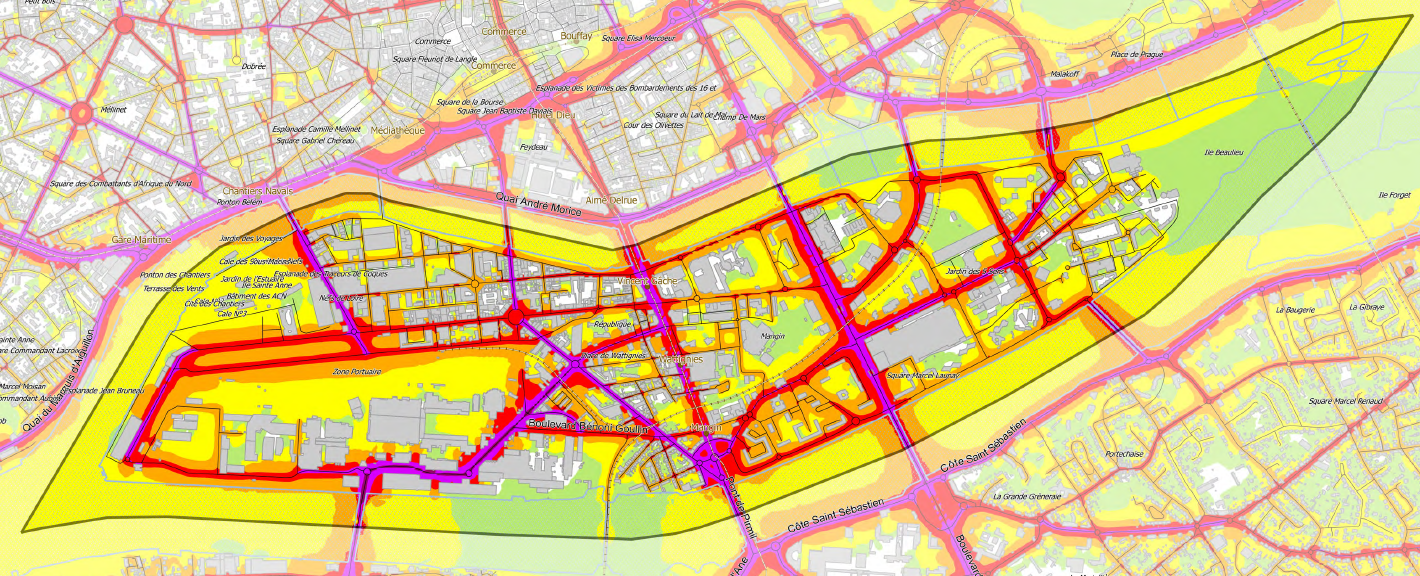
\includegraphics[width=0.7\linewidth]{./figures/cartographie/Lden_ile_Nantes.PNG}}
\subfigure[\label{fig:ln}]{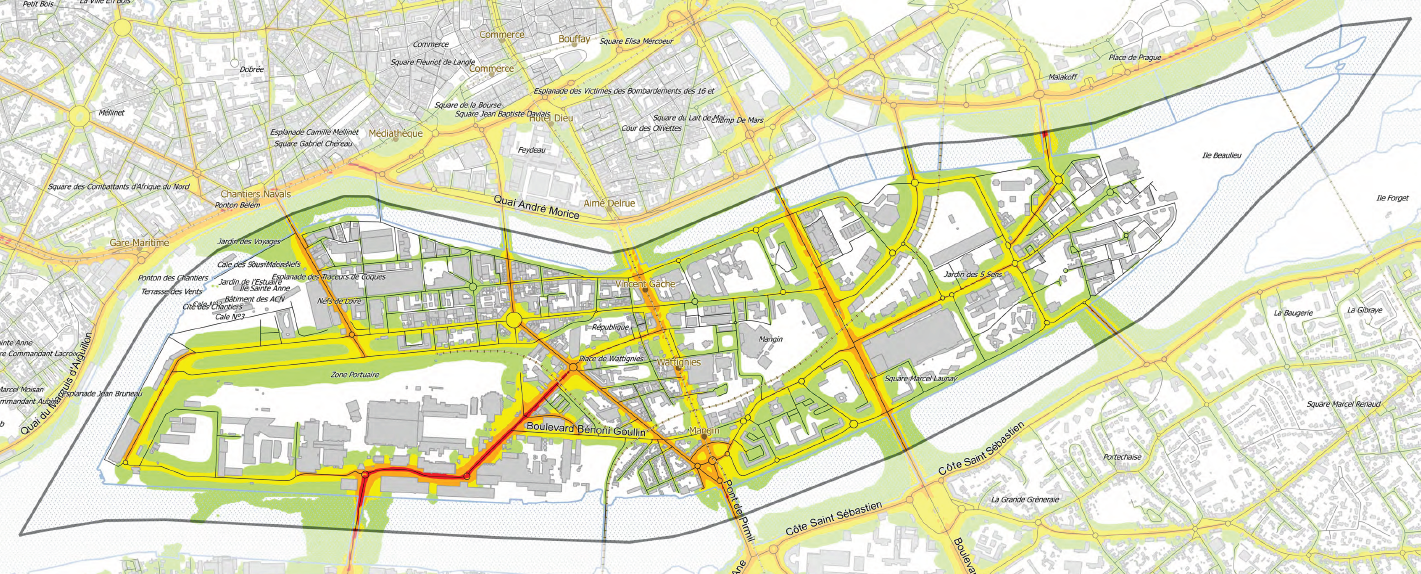
\includegraphics [width=0.7\linewidth]{./figures/cartographie/Ln_ile_Nantes.PNG}}
\caption{$L_{DEN}$ \subref{fig:lden} et $L_N$ \subref{fig:ln} de l'île de Nantes pour le trafic routier \cite{nantes_carte}}
\label{fig:carto_nantes}
\end{figure}

Ces cartes sont issues de calculs numériques qui nécessitent de définir, comme données d'entrée, les caractéristiques des sources sonores et de l'environnement.  Dans le cas du trafic routier, cela revient à déterminer : 

\begin{itemize}
\item les vitesses des véhicules sur les portions de routes principales, 
\item les débits de véhicules (nombre de véhicule par jour), \item la composition du trafic (nombre de poids légers et de poids lourd).\\
\end{itemize}

Des lois d'émissions sont alors calculés. En déterminant la topographie de la ville (architecture, revêtement du sol) et en obtenant les conditions météorologiques moyennes (température, vent), il devient possible de calculer avec l'aide de modèles numériques de propagation acoustique, les niveaux sonores dans la villes produites par ces sources sonores. Plusieurs modèles existent comme le modèle NMPB-routes-2008 \cite{setra_prevision_2009-1, setra_prevision_2009-2},  CNOSSOS-EU \cite{CNOSSOS}, RSL-90\dots{} La génération des cartes peut être réalisée par des logiciels du commerce comme Mithra, CadnaA, Immi\dots{} qui font alors le choix d'utiliser un modèle de propagation parmi ceux existant. Actuellement, la méthode CNOSSOS-EU est l'approche la plus couramment utilisée à l'échelle de l'UE. Mais à l'heure actuelle, ce sont les logiciels accompagnés d'un Système d'Information Géographique (ou GIS pour \textit{Geographic Information System} en anglais) qui offrent le plus de possibilité. Un GIS est un système informatique conçu pour stocker, analyser et manipuler plusieurs type de données spatiales et géographiques comme l'architecture des villes ou le nombre d'habitants présents. Leur utilisation permettent ainsi d'améliorer la qualité des cartes et de mieux connaitre l'impact des niveaux sonores sur les citadins \cite{murphy2011scenario}. Par exemple, le logiciel OrbisGIS\footnote{\url{http://orbisgis.org/}}, destiné à représenter de données spatiales, permet la réalisation de cartes de bruit à l'aide de l'ajout d'un plugin, \textit{Noise Modelling}, développé par \cite{fortin:hal-00845701}. Un résumé des étapes est présenté en Figure \ref{fig:cartographie}.\\

\begin{figure}[t]
\centering
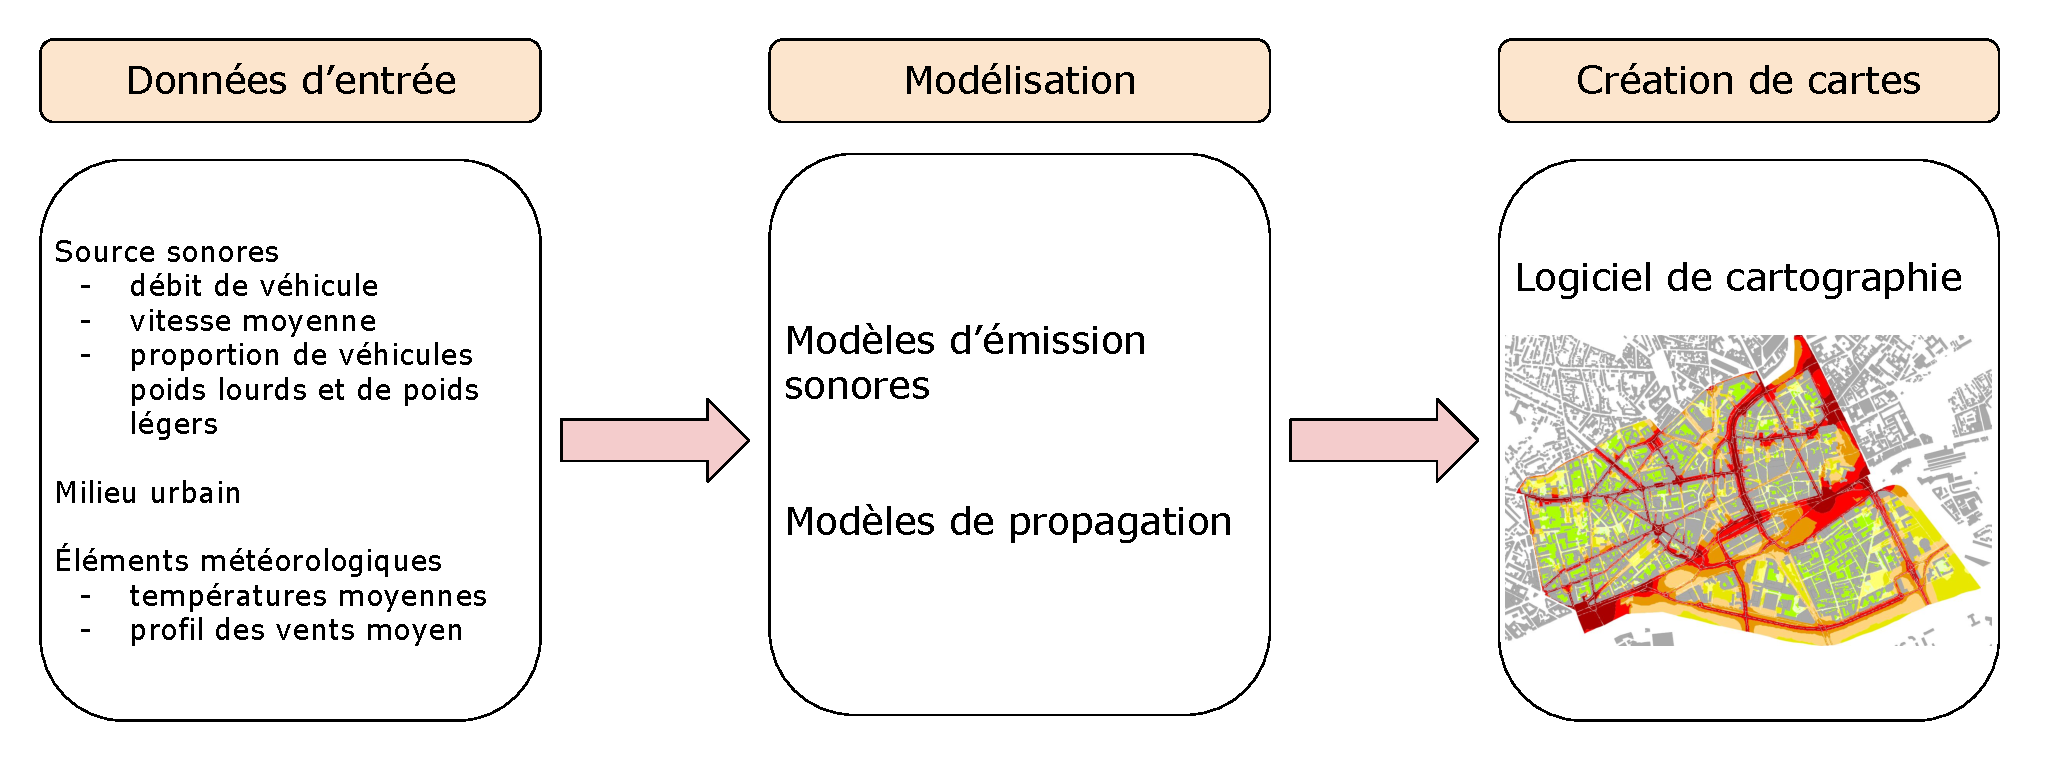
\includegraphics[width=.85\linewidth]{./figures/cartographie/cartographie.pdf}
\caption{Résumé des étapes menant aux cartes de bruit de trafic}
\label{fig:cartographie}
\end{figure}


De nombreuses études basées sur l'étude du bruit en ville ou sur la réalisation de cartes de bruit dans des quartiers utilisent comme référence la directive européenne \cite{murphy_environmental_2006, murphy_estimating_2009, Eriksson_residential_2013}. Cependant, si l'utilité de ces cartes n'est pas remise en cause, leur application ou les erreurs d'interprétations qu'elles peuvent engendrer sont toutefois questionnés.  

\section{Limitations des modèles prédictifs de bruit de trafic}

L'ensemble des différentes étapes qui permettent la génération de cartes de bruits est parfois discuté en raison des erreurs ou des incertitudes qu'elles peuvent induire. 

\subsection{Incertitudes sur les données d'entrée}

La première source d'erreur est naturellement celle venant de l'estimation des données d'entrée qui se propage par la suite aux étapes suivantes. 
Les grandeurs renseignées sont des moyennes qui induisent forcément des écarts types qui interagissent dans la suite des étapes. Le milieu urbain ensuite est simplifié (pour éviter de complexifier et diminuer le temps de calcul) simplifiant aux bâtiments, l'influence des plus petits mobiliers urbains est mise de cotés.
 

\subsection{Incertitudes des modèles physiques}

Ce type d'erreur est liée au choix de la méthode de calcul employée. Avant même la mise en place de la directive, Steele, dans \cite{steele_critical_2001}, avait comparé les méthodes de calculs (données d'entrée, type de cartographie, méthode de propagation des différents logiciels). Parmi cette diversité d'outils, l'auteur met en avant le problème, soulevé également par \cite{king_implementation_2011}, de la diversité des outils et des méthodes de calculs qui peuvent être employées. Plus récemment, Garg et Maji \cite{garg_critical_2014} réalisent une comparaison entre 8 méthodes de calcul (FHWA, CoRTN, RLS-90, ASJ RTN, Harmonoise, Son Road, Nord 2000n NMPB-Routes-2008) selon de nombreux points techniques : 

\begin{itemize}
\item modélisation des sources sonores (trafic, ferroviaire), 
\item condition de trafic (constantes, accélération/décélération, intersection\dots), 
\item modèle de propagation, 
\item prise en compte de la divergence géométrique, 
\item données d'entrées prise en compte, 
\item modélisation des effets de sol,
\item effets météorologiques,
\item effets de diffraction,
\item \dots  \\
\end{itemize}

Par exemple, la méthode RLS-90 est la seul à prédire la densité de trafic sur les axes routier. La catégorisation des véhicules varient également entre les méthodes : dans la méthode Nord-2000, les véhicules sont divisés en 3 catégories selon leur poids alors que dans Son Road, il n'y en a que 2. Dans le cas du modèle de propagation, Harmonoise propose 3 méthodes (équation parabolique, tir de rayon et éléments de frontières) afin de s'adapter à différentes configuration là où, dans FHWA, c'est l'équation de propagation qui est résolue en prenant en compte des phénomènes comme l'absorption atmosphérique, les impédances des différentes surfaces rencontrées\dots{} Enfin les effets météorologiques sont pris en compte dans la méthodes NMPB qui suppose des conditions homogènes et favorables à la propagation. Dans Nord 2000, les gradients de température et de vent sont inclus alors que, dans les modèles Son Road et CoRTN, ces phénomènes ne sont pas pris en compte. L'ensemble des ces points amènent donc à des résultats divergeant entre les méthodes. 
L'auteur conclut enfin qu'il est toutefois difficile de déterminer un \og meilleur \fg{} modèle par rapport aux autres car chacun prend en compte des phénomènes qui ne sont pas décrit par d'autres méthodes. La validation de ces modèles par la mesure \textit{in situ} est complexe puisque de nombreuses sources sonores qui ne sont pas modélisées sont présentes en villes. 

Il est donc nécessiaire d'utiliser une méthode harmonisée à l'échelle européenne afin de pouvoir comparer les cartes de bruits des villes. Pour cela, la méthode CNOSSOS-EU \cite{CNOSSOS} a été développée.

\subsection{Incertitudes liées à la modélisation numérique}

Les cartes de bruits étant simulées numériquement, des problèmes apparaissent également lié à la modélisation et à la discrétisation du milieu urbain. Afin de limité la durée des calculs de techniques d'optimisation sont utilisées comme la discrétisation du milieu mais aussi des sources de bruits. Par exemple, pour une route décrite comme une source linéique de bruit, celle est discrétisé en un ensemble de source ponctuel alignées. Le choix de la distance entre ces points est alors un compromis à faire entre temps de calcul et précision souhaitée. Toutefois la position de ces sources influe ensuite sur les phénomènes de réflexion et de diffraction. De plus, toujours pour réduire les temps de calculs, les niveaux sonores entre les points calculés sont déterminés au moyen d'un calcul d'interpolation (méthode de Krigeage) qui viennent donc rajouter en plus des incertitudes \cite{van_leeuwen_noise_2015}. 

\subsection{Incertitudes liées à la restriction d'informations}

Une des principales limites des modèles de bruits en ville est la restriction d'informations qu'elles proposes : seul 2 niveaux sonores, $L_{DEN}$ et $L_N$, par source de trafic, sont estimés et mis à jours seulement tous les 5 ans. Cependant, le trafic routier, ferroviaire et aérien varient aussi bien à l'échelle de l'année, d'une journée ou même d'une heure \cite{lv2015traffic}. Résumer l'ensemble de ces variations à 2 niveaux sonores équivalent est donc très restrictif. 
Une piste pour contourner cette limite est la création de cartes de bruits dynamiques basé sur un modèle dynamique du trafic routier qui permet de mieux simuler les flots de véhicules. 

Le choix des niveaux sonores pondérés équivalent est aussi sujet à caution : si pour le bruit de trafic celui-ci peut s'apparenter à un bruit de fond, dans le cas du trafic aérien  car il atténue les niveaux sonores crêtes qui sont beaucoup plus marquant pour cette source de bruit pour le riverain.

Enfin, ces modèles prédictifs ne sont pas actuellement validé \textit{in situ}. 
En effet, ces modèles de bruits actuel ne permettent d'estimer que les niveaux sonores des sources relatifs au trafic alors que le milieu urbain est composé d'une multitude de sources sonores qui ont une influence sur l'ESU perçu par le citadin.\\ 
\subsection{Vers la modélisation d'autres sources sonores ?}

La réalisation de cartes avec les modèles actuels restent un processus complexe et couteux. Si la réalisation de ces cartes restent un outils indispensable pour mieux connaitre l'impact du bruit sur les citadins, les incertitudes quant aux données d'entrée et au modèles de sources de propagation peuvent mener à des mauvaises estimation des niveaux sonores et donc à ne pas adapter les bonnes résolutions pour réduire ce bruit. 
De plus, il est complexe de valider ces modèles par des mesures afin de s'assurer de la cohérence des résultats calculé. De précédente études \cite{Mioduszewski, zannin_characterization_2013} ont montré qu'entre les mesures et les calculs, des différences sont observées. Si ces différences peuvent provenir des inexactitudes généré par la simulation, une part de ces écarts provient de la présence d'autres sources sonores qui sont prise en compte dans les mesures mais qui ne sont pas modéliser. En effet, les modèles prédictifs actuels de bruits permettent d'estimer les niveaux sonores des sources les plus gênantes et bruyantes mettant de coté de nombreuses autres sources sonores qui ont pourtant une influence sur la perception des ESU par le citadin. La validation de ces modèles numériques par rapport aux mesures n'est donc pas si trivial. 

La modélisation d'autres sources comme les voix, les oiseaux ou les fontaines, des éléments connotés le plus souvent positivement, n'est, pour l'instant, pas réalisé. 
Ces sources sont donc mise de coté parce que non prise en compte dans les textes normatifs qui se concentrent sur les sources plus prépondérantes et gênantes. Leur modélisation est possible mais peu étudié pour l'instant. La difficulté pour ces sources revient d'abord à les localiser pour cibler les emplacements où leur influence sur l'ESU est prépondérante. En effet, là où les éléments trafic se concentrent sur les axes qui leur sont dédiés, les sources comme les piétons et les oiseaux sont plus difficiles à déterminer car plus disparate. Il est cependant possible de déterminer statistiquement où ces sources sont le plus susceptibles de se trouver (sur des places ou sur les trottoirs pour les piétons, dans les parcs pour les oiseaux). Mais ces sources restent mobiles et peuvent se diffuser dans toute la ville et la quantité d'individu reste difficile à estimer. À l'inverse, d'autres sources sonores, comme les fontaines ou les cloches d'une église, sont plus faciles à localiser car fixes. Un second aspect est lié à la modélisation des émissions sonores de ces sources. il existe peu ou pas de modèle dans la littérature qui permettent de décrire les formes spectrales de ces sources. Dans \cite{hayne2011prediction}, un modèle de bruit de foule moyenne est proposé permettant d'estimer le niveau de puissance acoustique. L'influence de la taille de la foule, de l'âge ou encore de l'orientation de la foule est également évoquée. \\


L'utilisation de modèles prédictifs n'est donc pas suffisant pour définir les ESU. Les modèles existants se concentrent sur les sources de bruits de trafic, certes prépondérants, mais qui ne permettent pas définir un ESU dans son ensemble. L'absence de la prise en compte des autres sources, manque également mais reste toutefois compliqué à implémenter. 

Afin de considérer l'ensemble des sources et des évènements sonores présent en ville et de compléter l'apport des modèles prédictifs, une autre approche est envisagé basé sur la réalisation de mesures. 

\section{Utilisation de mesures acoustiques}

L'utilisation de mesures acoustiques en villes pour définir les ESU est de plus en plus courantes. Plusieurs approches sont possibles pour cela et sont l'objet d'études.

\subsection{Déploiement de réseaux de capteurs fixes}

Un des premier déploiement de capteurs a consisté à installer à des positions définies des microphones professionnels pour une durée finie. Cette approche permet ainsi d'avoir accès aux variation à long terme des niveaux sonores à l'emplacement des microphones.
Dans \cite{Mioduszewski}, ce sont 40 microphones qui sont placés isolément à travers la ville de Gdansk en Pologne pour une durée d'un an afin de valider la cartographie de bruit. Dans, \cite{zannin_characterization_2013}, c'est 58 points de mesures qui sont déployé dans un campus universitaire de la ville de Curitiba au Brésil afin d'étudier son environnement sonore. Mais grâce au développement de capteurs acoustiques à bas coûts \cite{van2010use}, il devient, aujourd'hui, envisageable de déployer un plus grand nombre de microphones à travers les villes pour des durées plus longues. 

CARTE AVEC RESEAUX MICROPHONES (CENSE)

\`A l'heure actuel, plusieurs projets étudient la mise en place et la faisabilité de telle installations comme le projet italien DYNAMAP \cite{dynamap_2016}. Ce projet a pour objectif de développer un système de cartographie de bruit dynamique basé sur des réseaux de capteurs à bas coûts installés en ville. Une application de ce projet a déjà été réalisé dans deux villes tests, Milan et Rome \cite{bellucci_life_2017}. 


En France, le projet RUMEUR \cite{mietlicki2012innovative}, en région parisienne, existe déjà depuis plusieurs années où des réseaux de microphones ont été déployé afin de mesurer le bruit aérien aux abords des aéroports. Un site internet\footnote{\url{http://rumeur.bruitparif.fr/}} permet alors au citoyen d'avoir un aperçu complet des mesures réalisées sur de nombreux sites et de voir l'impact de bruit aérien dans ces zones. Le projet CENSE\footnote{\url{http://cense.ifsttar.fr/}} vise à développer un réseau de capteurs dans la ville test de Lorient afin d'agréger les données simulées du niveaux sonores du trafic avec des mesures réalisées en villes ce réseau.  

L'installation de tels réseaux de capteurs nécessite de gére de nombreuses problématique techniques comme la disposition des microphones, leur maintenance, la transmission des mesures, leur alimentation\dots{}
Toutefois, la réalisation de mesures acoustique en ville n'est pas nécessairement obligé d'être réaliser via un réseaux de capteurs fixes. D'autres pistes sont également explorées.

\subsection{Mesures mobiles}
En parallèle des réseaux fixes, la mesure mobile est envisageable. Elle consiste à réaliser des mesures en plaçant le microphone sur un support mobile (piéton, cycliste, voiture, bus). L'avantage de cette méthode est sa capacité à pouvoir couvrir plus facilement une plus grande surface urbaine à moindre coût. Les mesures mobiles sous-entendent deux manières d'être réalisées : soit la mesure est réalisé alors que son support bouge \cite{alsina-pages_design_2016} et dans ce cas un traitement du signal doit être effectué pour prendre en compte le bruit émis par ce support, soit le support permet de déplacer le microphone pour faire ensuite des mesures fixes \cite{manvell_sadman_2004} ce qui simplifie simplifie la tâche mais qui nécessite plus de temps pour couvrir une surface similaire par rapport aux mesures faites sur supports mobiles. 

Cette méthode permet toutefois de mieux résoudre les problème d'interpolation évoqué pour les mesures fixes. Dans \cite{can_measurement_2014}, à partir de mesures fixes, 2 méthodes classiques d'interpolations (méthode de distance pondérée inverse et méthode de Krigeage) sont testées et comparées à l'interpolation produite avec des mesures mobiles. Il en résulte que l'apport des mesures mobiles diminue l'erreur produite par rapport aux méthodes d'interpolation en cela qu'elles permettent d'apporter beaucoup d'informations quant aux variations spatiales du niveau sonore (rues calmes peu fréquentées, rue très passante) et aux variations spatiales provoquées par le trafic (intersection, tramway, rues piétonnes\dots) ce que ne permet pas une méthode d'interpolation numérique.

\subsection{Mesures participatives}
Enfin, dans le but de toujours plus sensibiliser le citadin à son environnement sonore, leur participation peut être sollicitée aux travers de mesures participatives. Celle-ci peuvent se réaliser en équipant les personnes de dispositifs spécifiques \cite{aumond2017study} ou bien à partir d'applications développées pour smartphones. Profitant de la démocratisation de ces appareils et de l'augmentation de leur performances, ces applications leur permettent d'avoir un dispositif performant pour mesurer les niveaux sonores dans leur poche. Cette approche permet surtout d'obtenir un plus grand nombre de mesures qui ont le plus souvent une distribution spatiale et temporel plus aléatoire mais qui sont aussi moins effectuées régulièrement. L'utilisation de ces mesures est toutefois encore sujet à caution puisque de nombreux problèmes sont à résoudre : calibration et performances des microphones dans les faibles et forts niveaux sonores, qualité de la réalisation de la mesure par l'utilisateur\dots{} Dans ce cas, le traitement statistique des résultats est un enjeu majeur afin de pouvoir utiliser correctement les résultats de ces mesures et de détecter les mesures incongrues \cite{guillaume2016noise}. Plusieurs applications ont été dévelopées comme NoiseSpy \cite{kanjo_noisespy_2010} ou Ambicity \cite{ventura2017estimation}. On peut également relever le projet \textit{Noise Planet}\footnote{\url{http://noise-planet.org}} qui a pour objectif de proposer un outil libre et gratuit pour évaluer le bruit de l'environnement sonore. Il comprend un application pour smartphone, NoiseCapture \cite{guillaume2016noise}, qui permet là aussi à l'utilisateur d'évaluer les niveaux sonores l'entourant tout en ayant la possibilité de décrire à l'aide de mots-clés prédéfinis les sons présents et l'ambiance sonore de la scène. La géo-localisation et les mesures sont ensuites collectées puis traitées par le système OnoM@p \cite{bocher_onomp_2016}. Puis dans une troisième étape, l'outil \textit{Noise Modelling} permet, à partir de ces mesures et informations de générer des cartes de bruits, publiées en ligne (voir Figure \ref{fig:carte_noiseModelling}).\\ 

\begin{figure}[t]
\begin{center}
    \begin{minipage}[t]{0.3\textwidth}
        \centering
        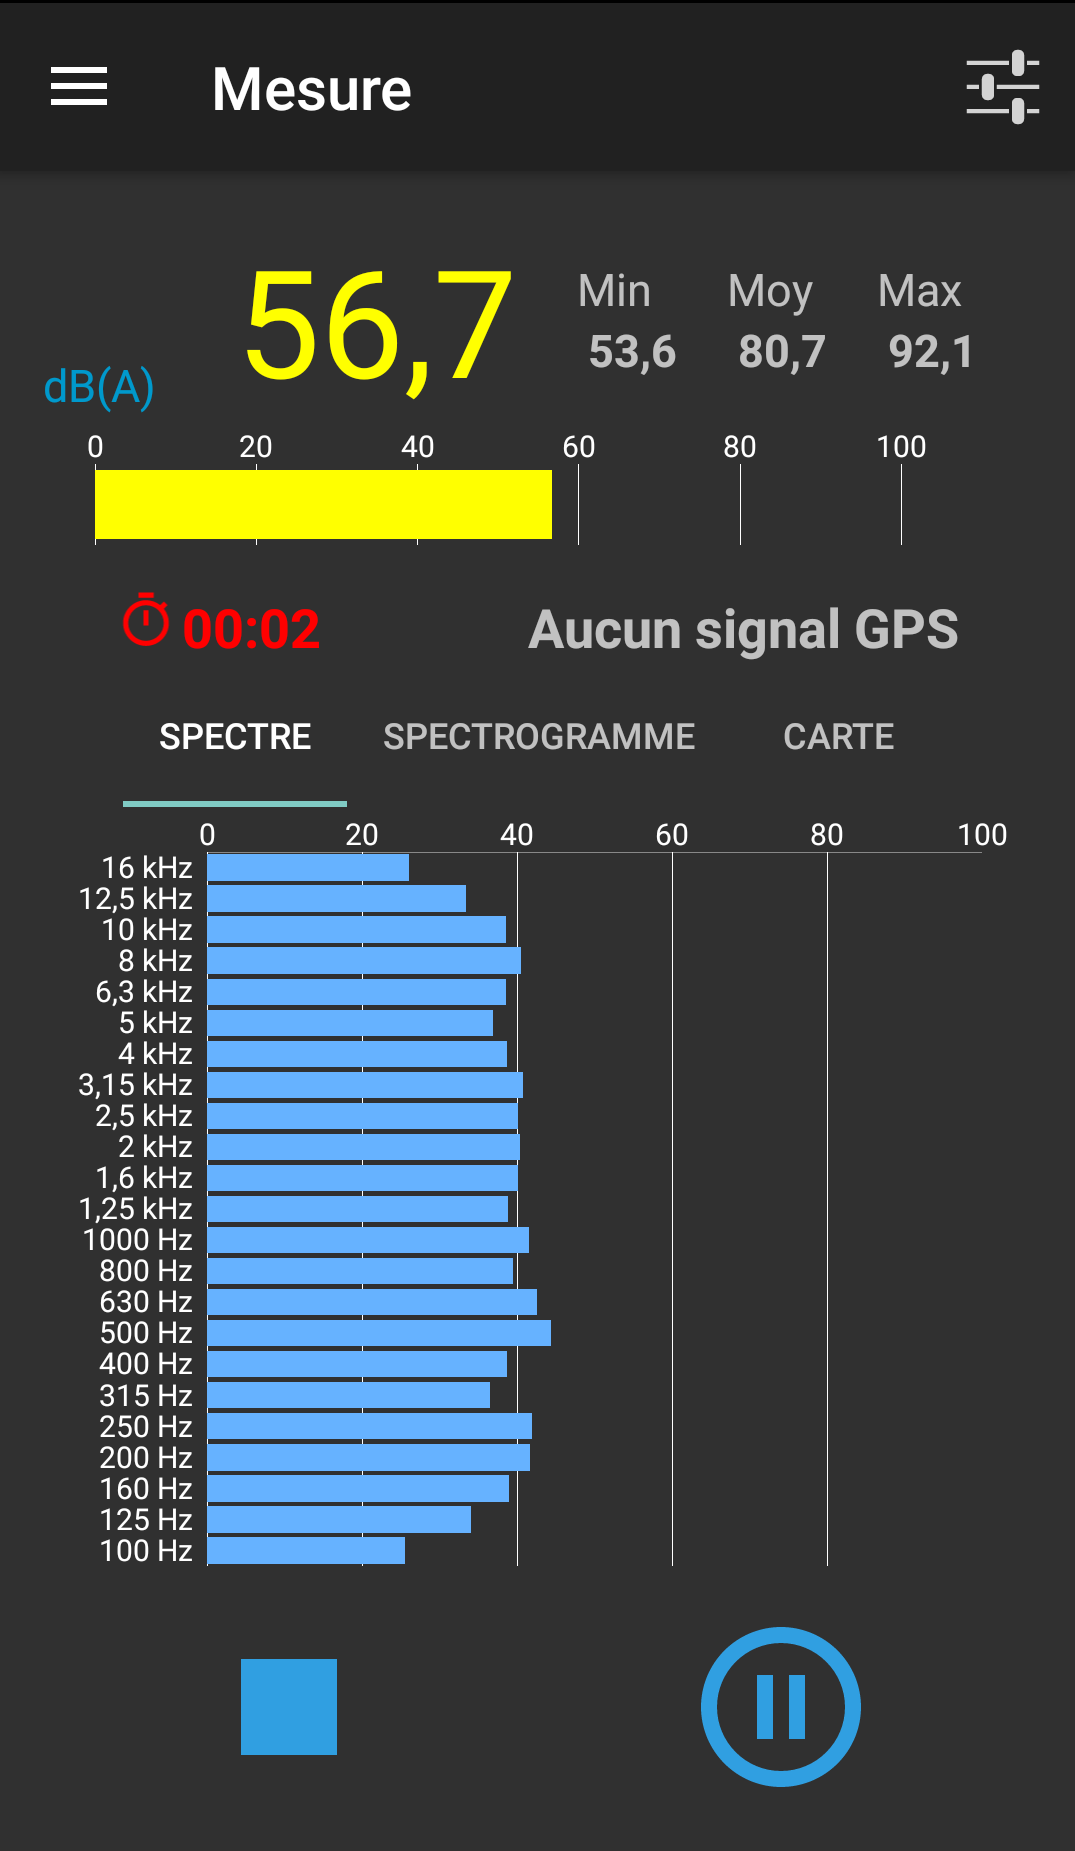
\includegraphics[width=0.9\textwidth]{./figures/autres/noiseCapture1.png}
    \end{minipage}
    \begin{minipage}[t]{0.3\textwidth}
        \centering
        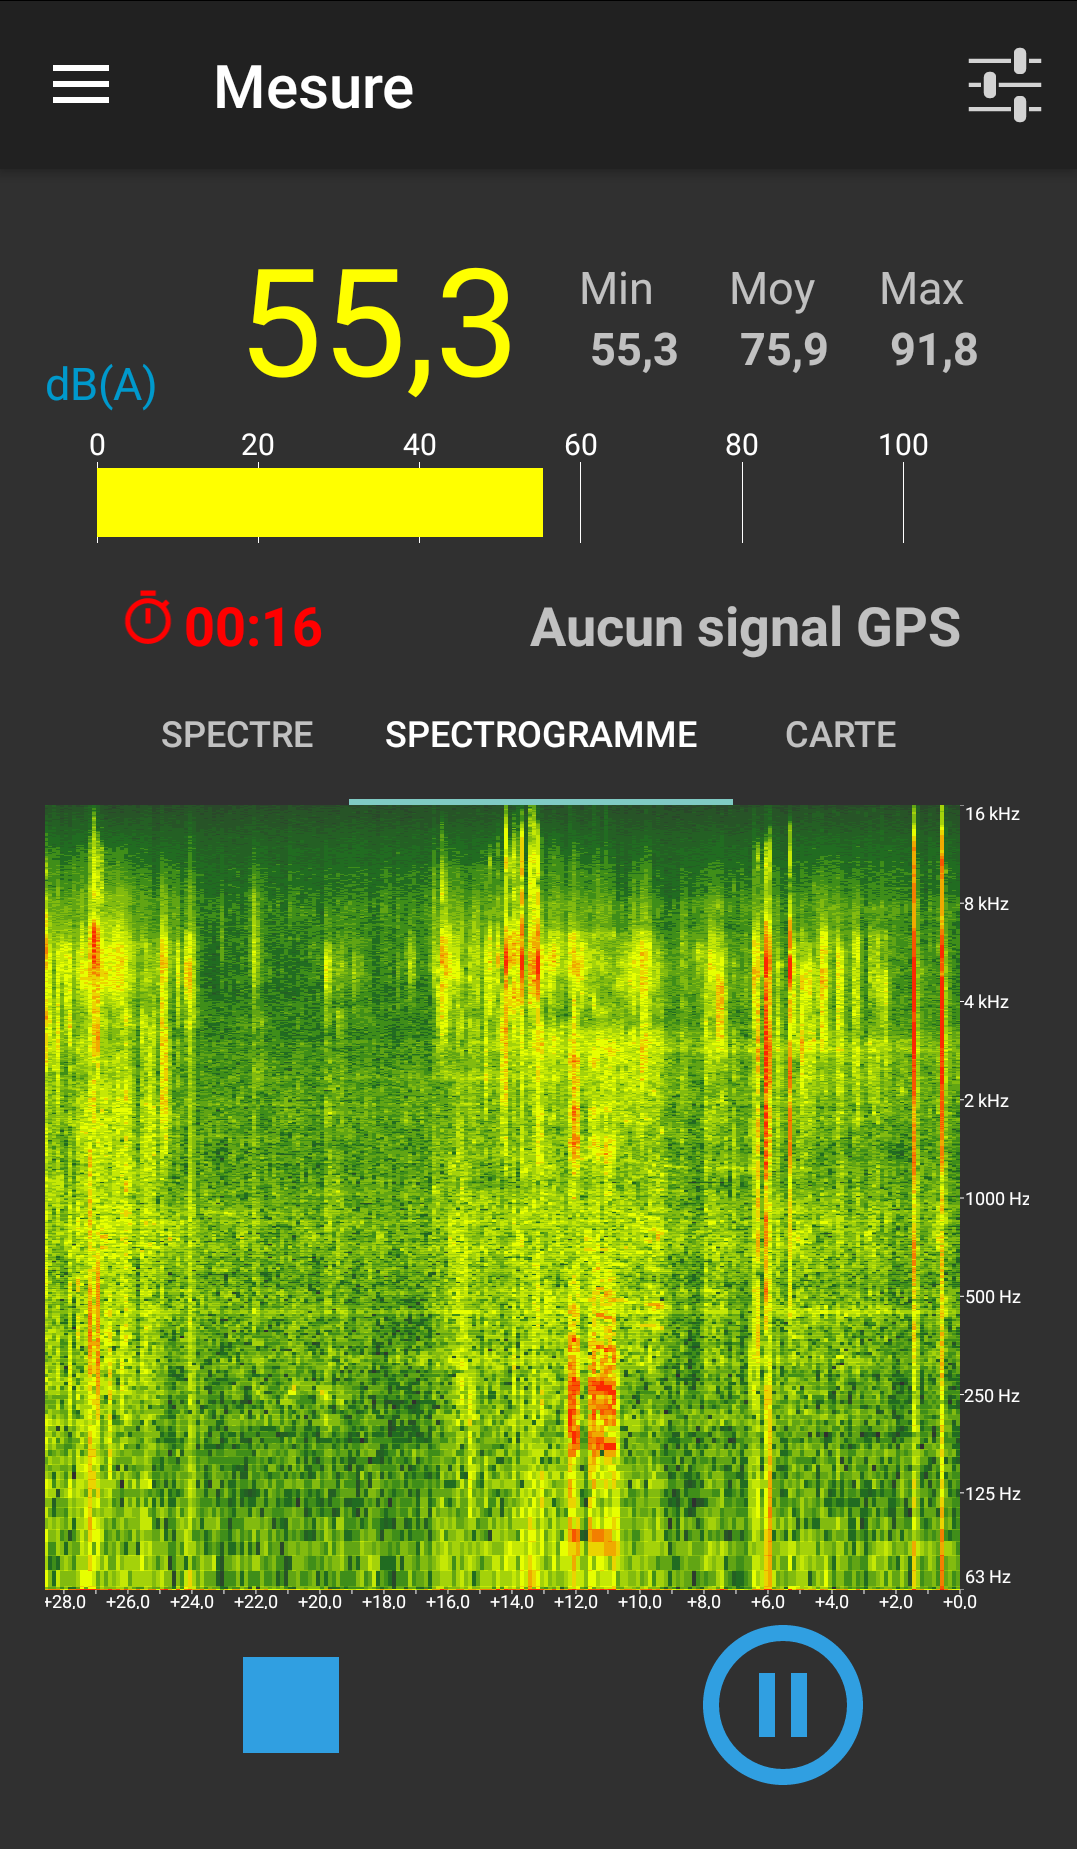
\includegraphics[width=0.9\textwidth]{./figures/autres/noiseCapture3.png}
    \end{minipage}
    \begin{minipage}[t]{0.3\textwidth}
        \centering
        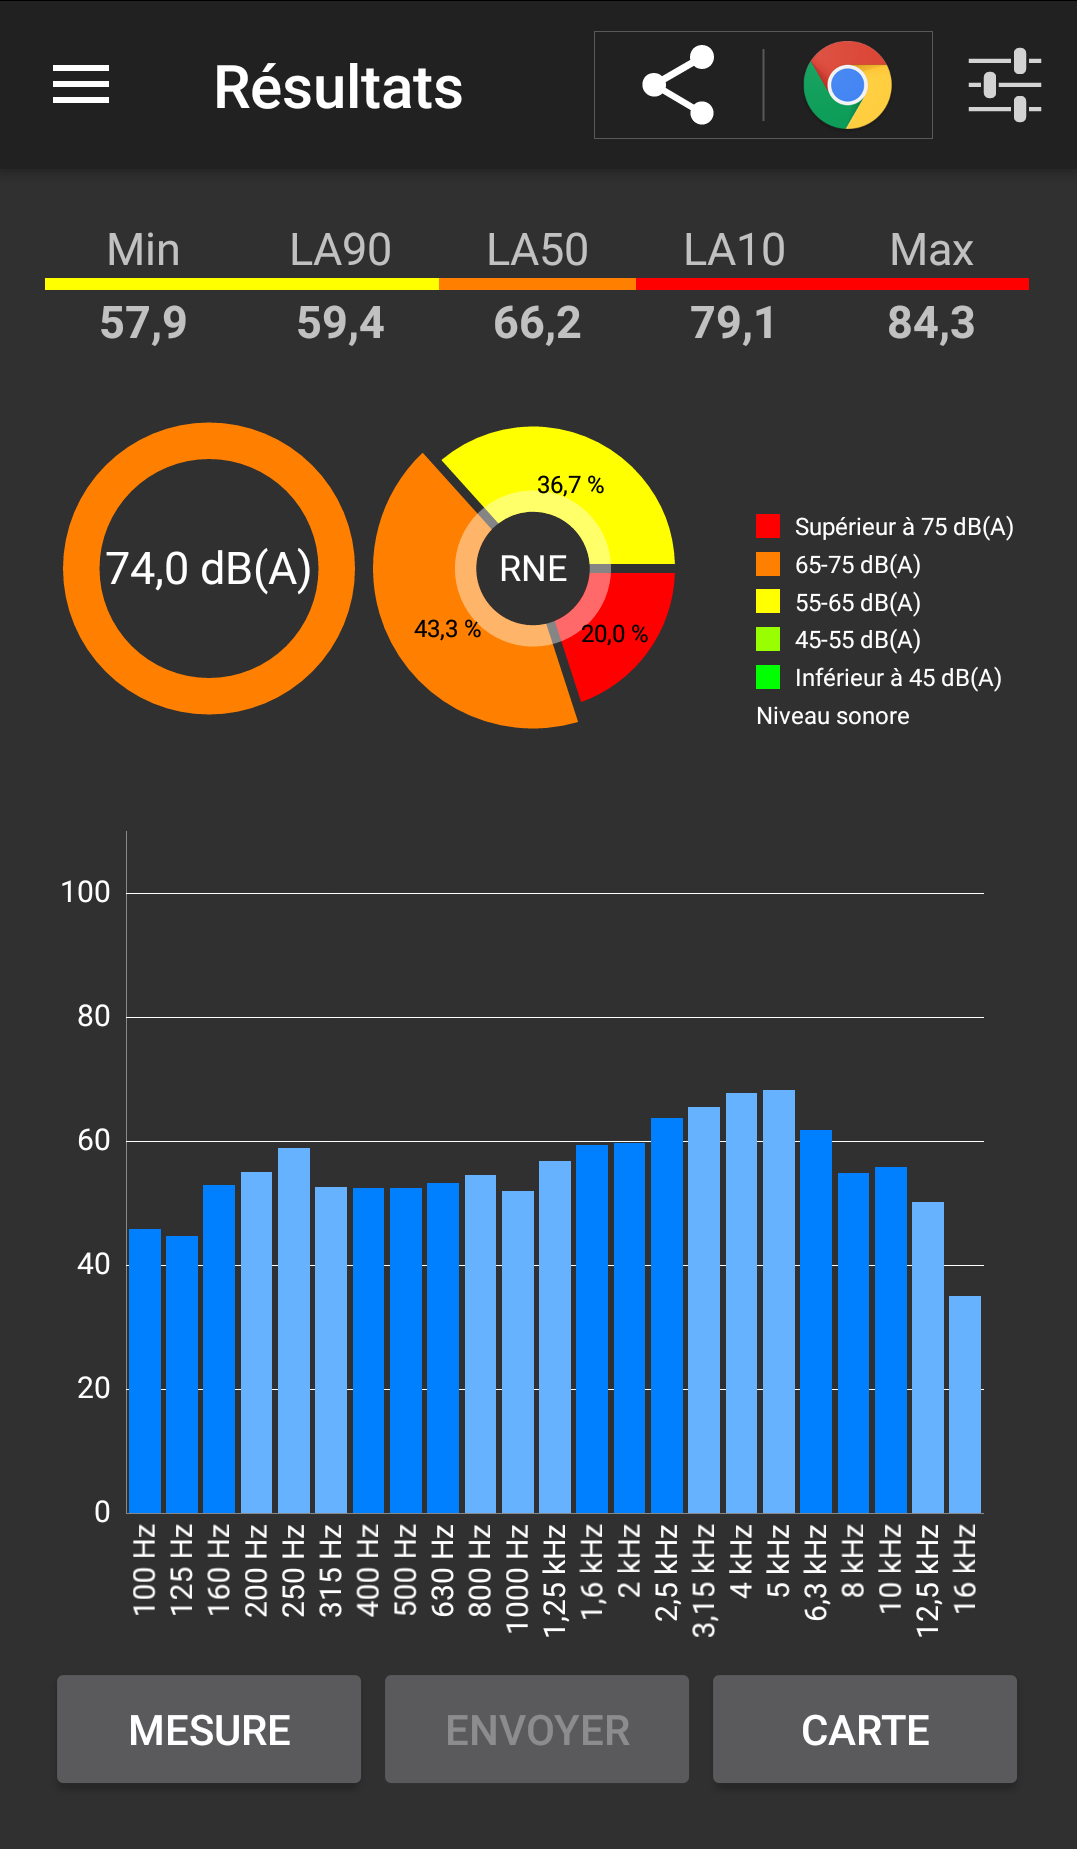
\includegraphics[width=0.9\textwidth]{./figures/autres/noiseCapture2.png}
    \end{minipage}
    \caption{Captures d'écran de l'application \textit{NoiseCapture}}
\end{center}
\end{figure}


\begin{figure}[t]
\centering
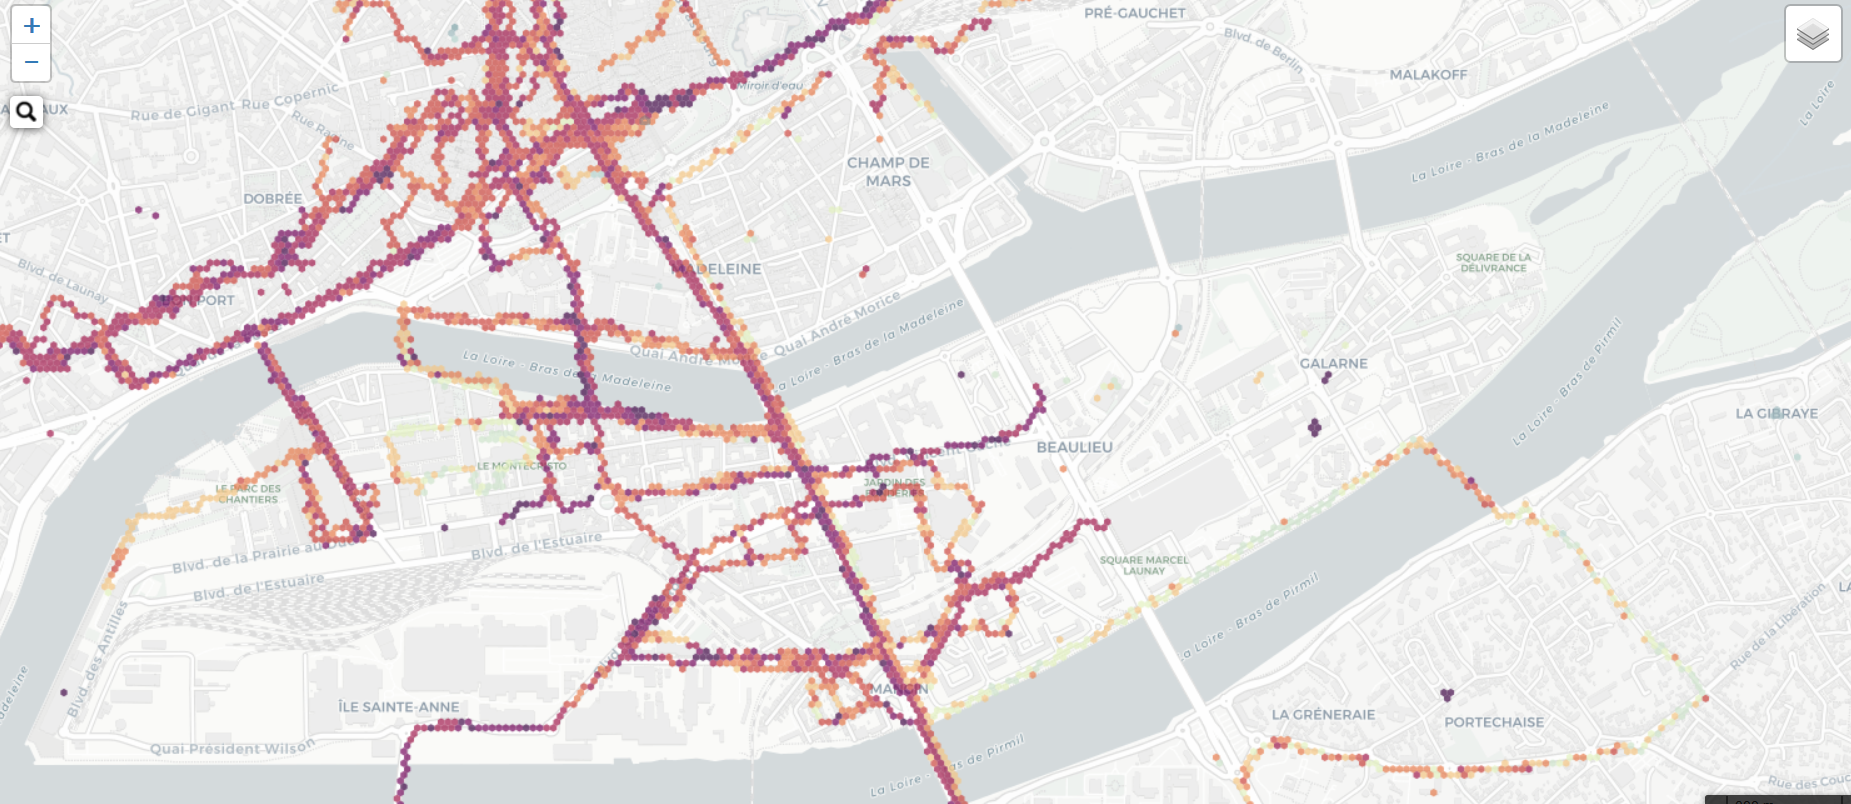
\includegraphics[width=0.7\linewidth]{./figures/cartographie/noise_modelling.PNG}
\caption{Carte de l'ESU de l'île de Nantes mesurée par l'application NoiseCapture  (relevée le 22/03/2018)}
\label{fig:carte_noiseModelling}
\end{figure}

Ce déploiement et cet utilisation de réseaux de capteurs s'insèrent dans le développement des villes dite intelligentes (\textit{smart city} en anglais). En effet, actuellement de nombreuses villes s'équipent en réseaux de différents types de capteurs disséminés dans le milieu urbain afin de mieux contrôler en temps réel de nombreux aspects de la ville : distribution d'énergie, gestion des transports, de l’eau ou des déchets. L'objectif étant alors d'optimiser le fonctionnement de la ville afin d'améliorer la qualité de vie des citadins. L'accès à ces données est rendu possible grâce au développement des réseaux de communication numérique, via Internet. La transmission d'informations par des réseaux, comme la 4G ou bluetooth facilitent l'échange et le partage des données mesurées et participe à la construction de l'Internet des choses (\textit{Internet of Things} en anglais) \cite{zanella2014internet}. Les applications de ces mesures et de ces réseaux, dans le cadre de la description des ESU, sont alors nombreux. 

\section{Applications des mesures}

\subsection{Cartographie du bruit de trafic}

Une des difficultés quant à l'utilisation de réseaux de capteurs fixes est celle de de la spatialisation des mesures et de la surface couverte par ces mesures : un réseau distribué selon un maillage dense permettra une bonne représentation de l'espace mais coutera cher à installer et à maintenir alors qu'une faible densité de capteur apportera peu d'information et nécessitera des interpolations entre les mesures, sources d'incertitudes. Dans le projet DYNAMAP, les stations fixes sont dispersées dans toute la ville et installées à des endroits spécifiques où différents scénarios de trafic routier sont possibles (homogénéité du trafic, type de revêtement, type de trafic\dots). L'évolution du trafic sur un de ces axes modifie alors celui d'un autre axe similaire mais qui ne possède pas de capteurs. Dans le projet CENSE, les capteurs sont déployés à l'échelle d'un quartier. Différentes méthodes d'interpolations existent alors pour pouvoir estimer les niveaux sonores entre les microphones (méthode linéaire , kriging). \\

L'une des applications les plus courantes est celle dédié à l'amélioration de l'estimation du bruit de trafic en cela qu'elle est la source sonore principale en ville et la plus gênante. Le réseau de capteur mis en place dans le projet DYNAMAP a ainsi pour objectif de permettre la génération de cartes de bruits dynamiques à partir des mesures. Pour cela, chaque capteur est placé en fonction de certaines routes


Dans le projet CENSE, l'amélioration de la cartographie du bruit de trafic est aussi présente. L'approche est toutefois différente puisqu'ici, le projet consiste à utiliser des techniques d'assimilation de données en vue de compléter les cartes de bruits prédite avec les mesures. 

\subsection{Classification des environnements sonores}
D'autres études se sont intéressé à l'ESU de manière plus générale afin de catégoriser les ambiances sonores. La réalisation de mesures permettent la classification des environnements par ambiance à partir de différents indicateurs physiques comme dans \cite{can_describing_2015} où le niveau sonore équivalent pondéré A, son écart type et le centre de gravité spectrale entre les bandes de 50 Hz et 10 kHz sont considérés pour discriminer les ambiances sonores. Dans \cite{salamon2015unsupervised}, Salamon et Bello utilise un algorithme de k-moyenne sphérique en tant que classifieur. La cartographie de l'ESU selon des ambiances sonores défini est alors possible pour offrir une autre représentation de la ville. 

\subsection{Cartographie des ESU perçus}

De plus, les aspects perceptifs et \textit{soundscape} sont également étudiés en vue de d'obtenir une caracétérisation plus fine de l'environnement sonore urbain (\cite{can_describing_2015}, \cite{brocolini_measurements_2013})

Toutefois, la représentation des niveau sonores des sources les plus génantes à travers leur niveaux sonores équivalent pondéré A n'est pas jugé comme suffisant pour représenter l'ESU. En effet, celui-ci est resenti par le citadin et par la perception qu'il en a. Cette approche est résumée sous la notion de paysage sonore (ou \textit{soundscape} en anglais). Proposée par R. Murray Schafer \cite{schafer1977tuning}, cette notion consiste à considérer que la perception de l'ESU par le citadin est liée à sa construction sociale (âge, expérience, milieu social\dots), là où l'ESU est  le résultat de phénomènes physiques (source sonores, diffusion du son, réverbération\dots). En conséquence, plusieurs études ont chercher à lier la perception de l'ESU à des indicateurs physiques (niveau sonore pondéré, niveau sonore fractile\dots) ou des indictaurs du \textit{soundscape} (\textit{loudnss, sharpness, roughness, fluctuation strength}). 
Ces modèles prédictifs peuvent être établit à partir d'écoutes réalisées en laboratoire comme dans \cite{torija2013application} où le paysage sonore est décrit à partir de 14 indicateurs dont le facteur crête (rapport du niveau sonore maximum sur le niveau sonore équivalent à 15 minutes), le niveau sonore pondéré A contenant une réponse impulsionnelle ou les niveau sonores des bande de tiers d'octave de 125 Hz et 16 kHz.
Il est également possible de réaliser des marches sonores (soundwalk en anglais). Ces marches présentent l'avantage de présenter la représentation du monde la plus réaliste et ainsi d'avoir une validité écologique idéale mais ont l'inconvénient de présenter peut de contrôle sur les sources sonores. Dans \cite{aumond2017modeling}, la notion de pleasantness est  définit à partir de deux modèles : l'un perceptif et l'autre physique. Le modèle perceptif est établit à partir du niveau sonores globale et du temps de présence de plusieurs source sonore spécifiques : trafic, voix, et oiseaux. Le modèle physique est basé sur des indicateurs physiques tels que le niveau sonore fractile à $L_{50}$ à 1 kHz ainsi que de la variation normalisée en temps et en fréquence de la bande de tiers d'octave de 500 Hz et de 4kHz. Ces indicateurs permettent alors de représenter la présence des sources sonores du modèle perceptif. 
Le développement d'outil permettant l'estimation du temps de présence et le niveau sonore des sources prédominantes dans ces modèles est l'objet de ces travaux.

De ces différents modèles, réaliser des cartes de l'ESU perçu à partir des mesures issus des réseaux de capteurs serait alors envisageable et permettraient d'apporter une autre représentation de l'environnement sonore de la ville basée sur la perception du citadin et non sur les niveaux sonores physiques prédits des sources sonores les plus gênantes.

\section{De l'extraction d'informations des mesures}

La question principale à résoudre est alors : comment extraire les informations pertinentes des mesures acoustiques ?

L'ensemble de ces mesures fait fasse un problème qui est la gestion des données et la détermination d'informations extraites des mesures. L'ESU est un milieu complexe composé d'une multitude de sources variées (trafic routier, voix, oiseaux, klaxon, bruit de pas\dots). ces sources ont des allures temporels différentes qu'elle soient brèves (le retentissement d'un klaxon) ou longue (le passage d'une voiture) ainsi que des allures spectrales variés (dans les basses fréquences pour le trafic, dans les hautes fréquences pour le sifflement des oiseaux). L'ensemble de ces sources sont aussi susceptibles de se superposer. La création d'outil adapté à cet environnement pour reconnaitre ou détecter des sources spécifique n'est donc pas triviale. Dans le cas du trafic routier, s'il existe des endroits où celui-ci est quasiment prépondérant sur les autres sources sonores (périphérique, grand boulevard), il existe tout de même de nombreux endroits où il est moins présent et plus discret.
Considérer l'ensemble des mesures et des enregistrements sans distinction particulière entre les sources peut donc mener à des surestimation de son niveau sonore et donc à une mauvaise interprétation des mesures. 

Dans \cite{Mioduszewski}, la réalisation de mesures par 40 stations fixes durant 1 an révèle que les niveaux sonores mesurés sont supérieurs à ceux prédit par les modèles prédictifs. Si cette étude révèle l'influence des saisons ou même de la semaine sur les niuveaux sonores, ils rappellent que les mesures sont susceptibles d'inclure des bruits \og sociaux \fg{} qui peuvent provoquer cette surestimation mais également que les niveaux prédit ne permettent pas d'inclure des bruits provoqué par des véhicules se garant à proximité des capteurs. Ces travaux révèlent la nécessité qu'il y a à générer des outils adapté à la détermination du niveau sonore trafic à partir des mesures. 


\section{Estimation du niveau sonore du trafic routier à partir de mesures}

\subsection{Objectifs}
Puisque c'est la source de bruit la plus gênante et principale, nous nous intéressons d'abord à l'estimation du trafic routier à partir d'un réseau de capteurs.
Appliquer un traitement sur le signal d'enregistrement (44,1 kHz en format wav).

\subsection{Protocole expérimental}

Extraire le trafic routier par des méthodes de séparation de sources, d'autre méthodes existent mais on retient celle là pour des raisons explicité plus tard

\begin{figure}[t]
\centering
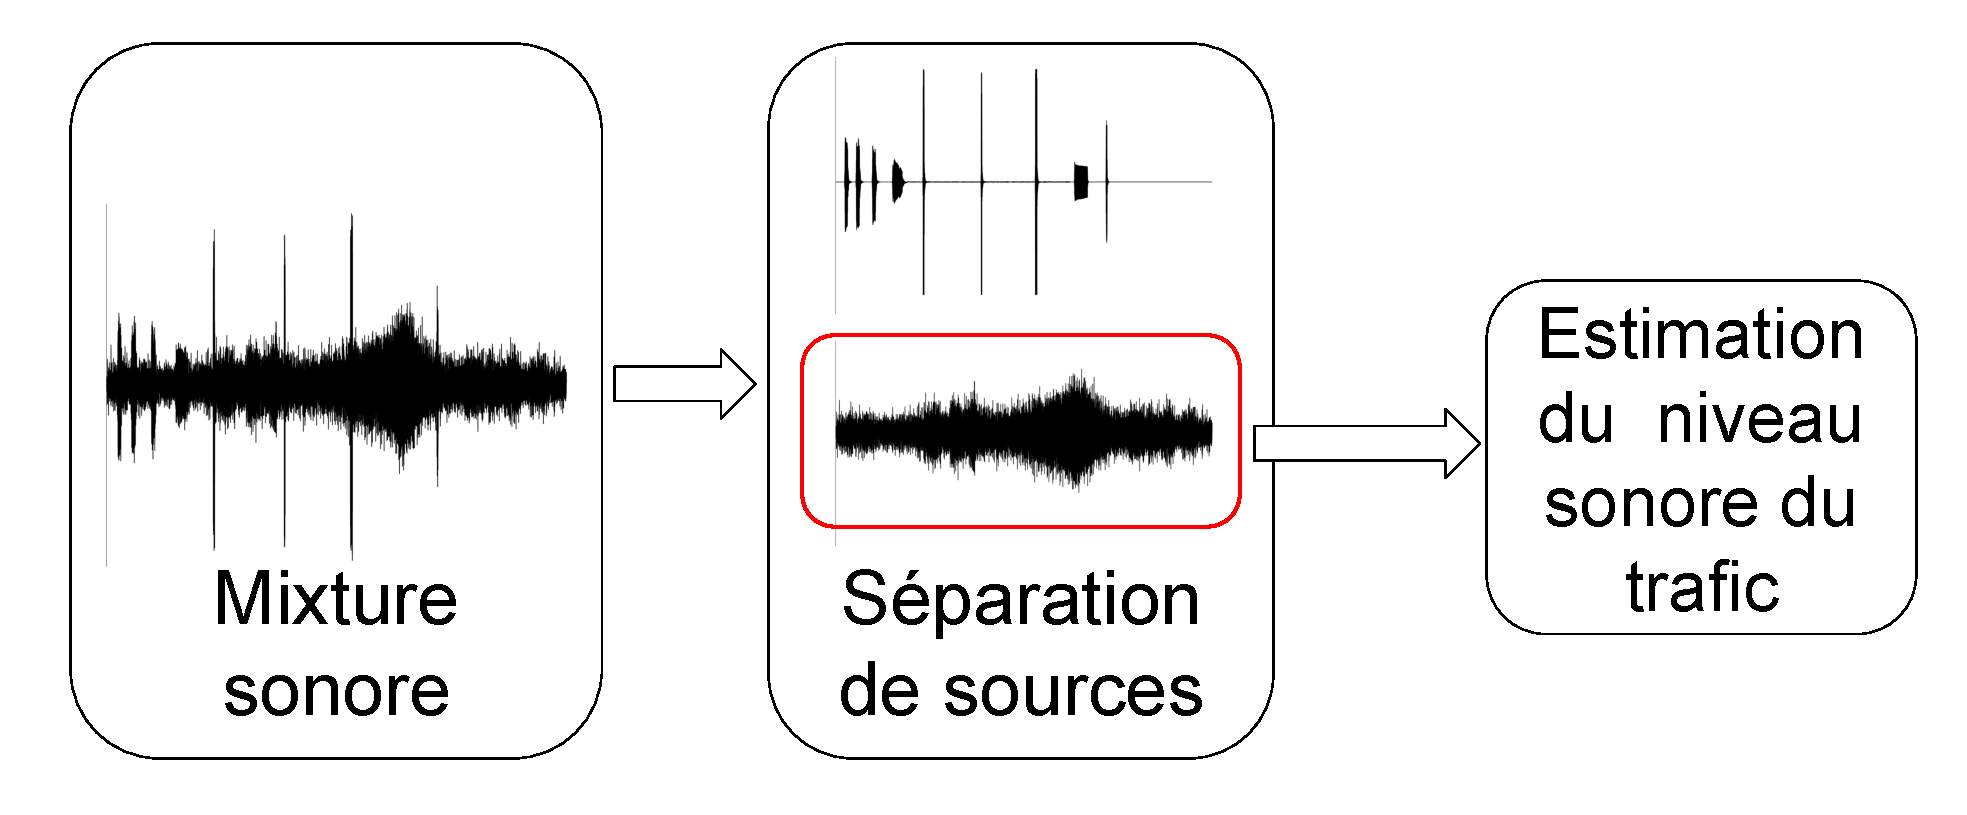
\includegraphics[width=0.7\linewidth]{./figures/NMF/bloc_diagram_source_separation.pdf}
\caption{Diagramme bloc de l'approche par séparation de sources.}
\end{figure}


Pour cela, l'utilisation d'enregistrement n'est pas possible puisque le niveau sonore du trafic réel est l'inconnu qu'on cherche. Dans le cas où il n'y a que du trafic, l'estimation fournie par la méthode peut être comparé mais quid des scènes sonores où le trafic n'est pas prépondérant et que d'autres sources sonores recouvrent cette composante ?
Le choix est donc fait d'appliquer la méthode de séparation de sources sur des scènes sonores simulées le plus réaliste possible. Cet aspect réaliste est primordiale afin de donner un sens et une validité aux résultats émis par la méthode.\\


Deux corpus de son sont construits. Le premier \textit{Ambiance} consiste en un ensemble de 6 sous-corpus où chaque sous-corpus mélange une composante \textit{trafic} avec une classe de son spécifique. Ces 6 classes de sons sont : \textit{alerte (klaxon, sirène), animaux (sifflement d'oiseaux, aboiement de chien), climat (pluie, vent, orage), humains (voix humaine), mécanique (bruit métallique, ventilation), transport (trains, avion, tramway)}. Pour chaque corpus, le niveau sonore du trafic est calibré suivant le niveau sonore de la classe de sons (appelée \textit{interférant} telle que rapport entre le niveau sonore en dB du signal \textit{trafic} et du signal \textit{interférant} (appelé $TIR$ pour \textit{traffic Interfering Ratio} en anglais) soit fixé : $TIR \in \lbrace$ -12 -6 0 6 12 $\rbrace$ dB avec 

\begin{equation}
TIR = L_{eq,trafic} - L_{eq,interférant}.
\end{equation}

Lorsque $TIR < 0$ dB, le signal trafic est plus faible que le signal interférant, à l'inverse lorsque $TIR>0$, le trafic devient la classe sonore prépondérante.
Le second corpus est composé à partir d'annotations d'enregistrement sonore réalisée en ville. 


Les scènes sonores étant simulée, un contrôle total des classes sonores présentes et de leur niveau sonore est alors possible. Les niveaux sonores exacte en dB sur la globalité de la scène pour chaque classe de son est ensuite disponible, dont le trafic, $L_{eq,trafic}$. En appliquant la méthode de séparation, la composante trafic est extraite du signal et son niveau sonore, $\tilde{L}_{eq,trafic}$, est estimé. La figure \ref{fig:diagramBlocProtocol}.

\begin{figure}[t]
\centering
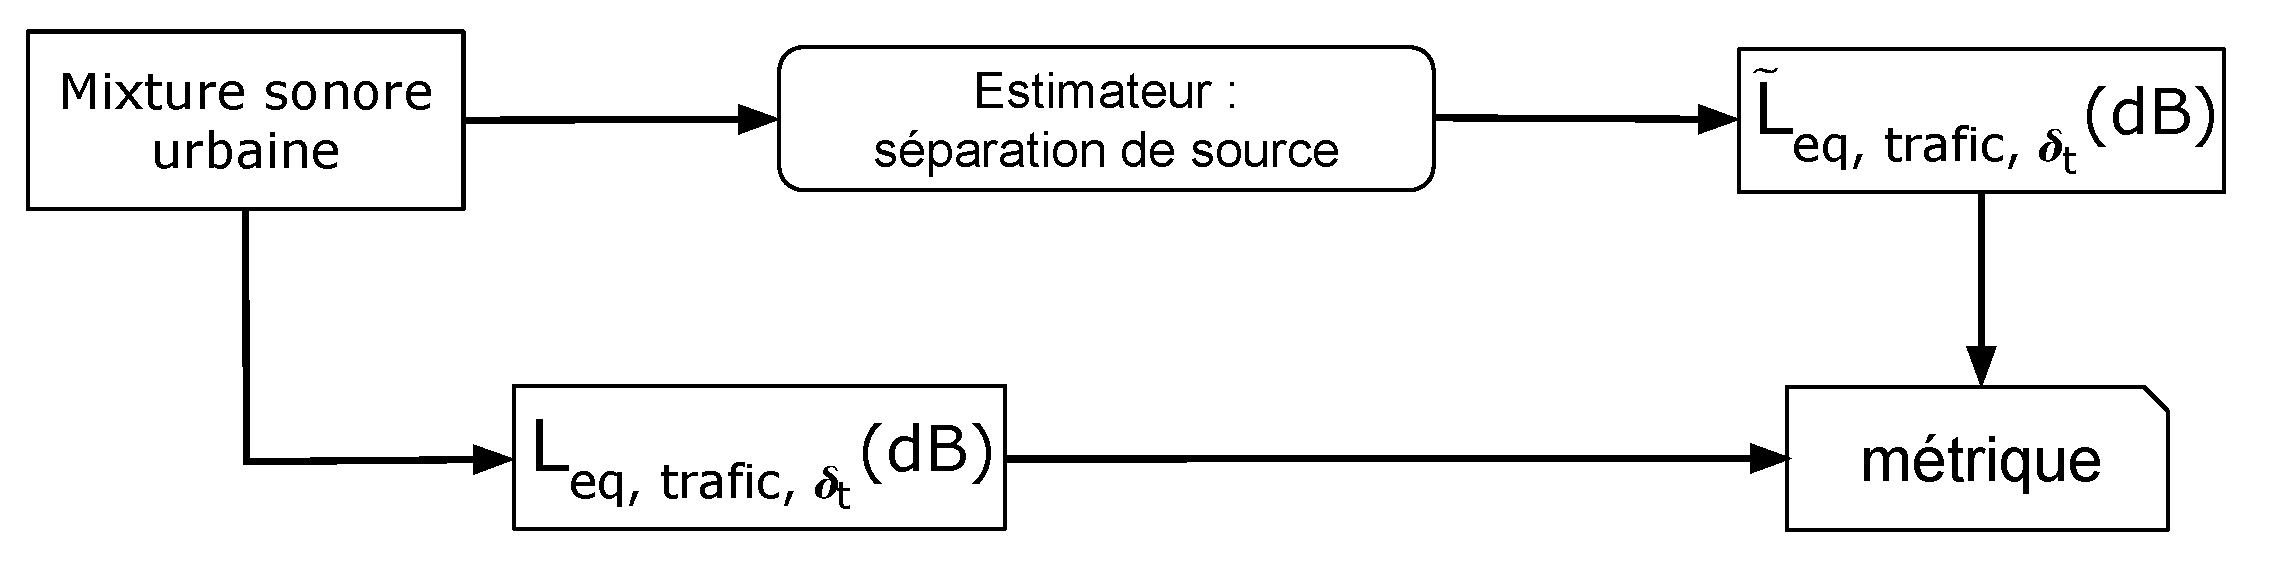
\includegraphics[width=0.7\linewidth]{./figures/NMF/Bloc_diagram_estimateur_FR.pdf}
\caption{Diagramme bloc du protocol expérimental.}
\label{fig:diagramBlocProtocol}
\end{figure}


Une métrique est alors choisie pour déterminer l'erreur moyenne produite sur un ensemble de $M$ scènes testés. Parmi les différentes métrique possible (somme des carrés des résidus $SCR$, racine de l'erreur quadratique moyenne $RMSE$), l'erreur absolue moyenne, $MAE$ (pour \textit{Mean Absolute Error}) est retenue,  

\begin{equation}
MAE = \frac{\sum_{i = 1}^{M} \vert L_{eq, trafic}^i - \tilde{L}_{eq, trafic}^i \vert}{M}.
\end{equation}

Contrairement à l'erreur RMSE, qui revient à la racine carré de la moyenne du carré des différences entre les données observées et réelles, qui pénalise plus les valeurs qui défie fortement, l'erreur $MAE$ présente l'intérêt de considérer un poids identique entre chaque différence et ainsi de gagner en interprétabilité.\\

Ces travaux se concentre sur l'estimation du signal du trafic routier tant elle est la source de bruit principale et la plus gênante. Toutefois, l'estimation d'autre signaux acoustique en ville est naturellement possible à partir de mesures acoustiques ou d'enregistrements en vue de détecter d'autres classes de sons spécifiques ou à l'étude plus générale de l'ESU.




%
%%\bibliographystyle{unsrt}
%%\bibliography{../bibliographie}
%%
%%\end{document} 
%
%%\subsection{Incertitudes liées à la modélisation numérique}
%%
%%Les cartes de bruits étant simulées, des problèmes apparaissent également lié à la modélisation et à la discrétisation du milieu urbain. Afin de limité la durée des calculs de techniques d'optimisation sont utilisées comme la discrétisation du milieu mais aussi des sources de bruits. Par exemple, pour une route décrite comme une source linéique de bruit, celle est discrétisé en un ensemble de source ponctuel alignées. Le choix de la distance entre ces points est alors un compromis à faire entre temps de calcul et précision souhaitée. Toutefois la position de ces sources influe ensuite sur les phénomènes de réflexion et de diffraction. De plus, afin de réduire les temps de calculs, les niveaux sonores entre les points calculés sont déterminés au moyen d'un calcul d'interpolation (méthode de Krigeage) qui viennent donc rajouter en plus des incertitudes \cite{van_leeuwen_noise_2015}. 
%%
%%IMAGE d'INTERPOLATION ?
%%
%%Enfin toujours en raison de la limitation des moyens numériques, l'effet de l'architecture urbaine (balcon, fenêtre) ou du mobilier urbain n'est pas pris en compte dans la modélisation des villes car trop complexe à réaliser alors que ces éléments ont un impact qui n'est pas pris en compte. 
%%
%%\subsection{Représentation des données et estimation du nombre de citadins touché}
%%
%%Une fois les cartes produites, indépendamment des remarques faites précédemment, une des critiques quant aux cartes de bruits est la limitation d'informations qu'elle produisent : un niveau sonore $L_{DEN}$ et $L_N$ pour décrire le niveau sonore du trafic. Ces deux seules indicateurs permettent certes d'avoir un aperçu global d'une grandeur qui, pourtant, évolue constamment. En effet, aussi bien à l'échelle de l'année ou d'une journée, le trafic routier évolue sans cesse. Cette évolution peut se diviser en 4 parties : un pic de trafic situé entre 7h et 9h et entre 16h et 18h correspondant au moment où les citadins emprunte leur voiture pour se déplacer entre leur domicile et leur travail. Entre ces 2 périodes, la quantité de voiture est plus faible \cite{}. La prise en compte ces évolutions de débit de trafic dans les modèles afin de simuler des cartes heures par heures est toutefois compliqué à mettre en œuvre car elle nécessiterait de grande quantité de ressources informatiques et cette approche ne permettrait pas d'obtenir l'évolution annuelle.
%%Coupler les modèles de sources et de propagation à des modèles dynamiques de trafic est une voie pour créer des cartes de bruit de trafic dynamiques prédictives. 
%%
%% Dans \cite{modiuszeski}, Modiuszeski compare le niveau sonore simulée prédit par la carte de bruit avec les résultats de mesures réalisée toute l'année. Il constate alors aisément que l'évolution des niveaux sonores évolue autant à l'échelle de la journée que de l'année rendant les valeurs $L_{DEN}$ et $L_N$ extrêmement restrictives. Enfin, au fur et à mesure que la perception du citadin de l'environnement sonore est mieux connu, il a été montré que les indicateurs de niveaux sonores du trafic pondéré A n'est pas suffisant pour rendre compte de sa perception de l'environnement sonore. Selon, le cadre architecturale de la ville, le statu social du citadin et les sources sonores présentes, pour un niveau sonore trafic similaire, l'agrément de l'ambiance sonore par le citatdin eut ne pas être la même. En conséquence, à partir des études sur le \textit{soundscape} \cite{schafer_soundscape_1993}, il peut être envisagé de réaliser des cartes de bruits, non plus liées à une seule source de bruit, mais à la perception du citadin de l'environnement sonore (\og agréable \fg{}, \og très désagréable \fg{}, \dots). Ces cartes ne se feraient plus alors à partir d'une source de bruit mais sur l'ensemble des sources sonores présentes dans les zones et permettraient, au citadin, de savoir si tel quartier a un environnement sonore agréable ou non.\\
%%
%%Des indicateurs de niveaux sonore, le nombre de citadins exposés au bruit peut être déterminé. Là encore, la méthode pour estimer ce chiffre est discutable. King et Murphy résument cela dans un paragraphe dans \cite{king_implementation_2011}. L'hypothèse faite est que les individus vivent et dorment toute l'année au niveau de la façade la plus exposée, ce qui n'est pas forcément représentatif de la réalité. Cette hypothèse conduit notamment à une surestimation du nombre de personnes touché par des niveaux sonores. \\
%%
%%La réalisation de ces cartes visant à diminuer l'exposition des citadins au forts niveaux sonores, les incertitudes provoquées par les différents étapes peuvent entrainer la mise en chantier d'un plan d'action mal adapté à la situation réelle. Mais l'amélioration des cartes, telles qu'elles sont faites actuellement, semble toutefois limité : l'augmentation de la résolution des permettrait bien de corriger certaines erreurs dû aux interpolations mais viendrait à augmenter considérablement les cout de calculs. De plus, ce choix rendrait impossible de mettre à jours les cartes régulièrement pour prendre en compte les fluctuations du trafic à l'échelle de l'année ou même encore durant la journée. En conséquence, à l'heure où les villes s'équipent en réseaux de capteurs (météorologique, qualité de l'air) en vue de devenir des \og villes intelligentes \fg{} (\textit{smart cities} en anglais), il devient possible d'ajouter des capteurs acoustiques afin de s'en servir pour décrire l'environnement sonore urbain. \\
%
%%Afin de mieux rendre compte de la perception du citadin, d'autre approche sont proposés qui passent notamment par la réalisation de marches d'écoute (ou \textit{soundwalk}). Cela  consiste à réaliser des parcours dans la ville où des auditeurs évaluent l'ESU à partir d'un questionnaire. Cette approche a été intiallement proposée par \cite{southworth1967sonic}. Le terme et la méthode a ensuite été popularisée par R. M. Schafer dans le concept du \textit{soundscape} où la pratique du \textit{soundwalk} est centrale dans l'étude de l'ESU \cite{schafer1969new, schafer1977tuning}. 
%%Cette méthode est ensuite rapidement repris par la communauté scientifique sous diverses approches : ces \textit{soundwalks} peuvent être mené par des passants ou bien par les chercheurs eux-mêmes, en groupe ou bien individuellement, avec des points d'arrêts d'écoute définie ou bien après avoir parcouru l'ensemble du parcours. 

%\subsection{Détection d'évènements sonore spécifiques}
%
%Plusieurs études se sont intéressées à la détection d'évènements particuliers en lien avec la sécurité. Par exemple, la détection acoustique de la sirène d'une ambulance est envisageable à partir d'un réseaux de capteurs \cite{schroder2013automatic,karpis2012system} ou bien de coups de feu ou d'explosifs \cite{showen1999automatic,simon_sensor_2004}.  
%Pour aller plus loin, \cite{foggia_audio_2016} propose de coupler des capteurs acoustiques à des caméra vidéo afin de faciliter la détection d'accident de la route. 